%%%%%%%%%%%%%%%%%%%%%%%%%%%%%%%%%%%%%%%%%
% Beamer Presentation
% LaTeX Template
% Version 1.0 (10/11/12)
%
% This template has been downloaded from:
% http://www.LaTeXTemplates.com
%
% License:
% CC BY-NC-SA 3.0 (http://creativecommons.org/licenses/by-nc-sa/3.0/)
%
%%%%%%%%%%%%%%%%%%%%%%%%%%%%%%%%%%%%%%%%%

%----------------------------------------------------------------------------------------
%	PACKAGES AND THEMES
%----------------------------------------------------------------------------------------

\documentclass{beamer}
\usepackage{booktabs}
\mode<presentation> {

% The Beamer class comes with a number of default slide themes
% which change the colors and layouts of slides. Below this is a list
% of all the themes, uncomment each in turn to see what they look like.

%\usetheme{default}
%\usetheme{AnnArbor}
%\usetheme{Antibes}
%\usetheme{Bergen}
%\usetheme{Berkeley}
%\usetheme{Berlin}
%\usetheme{Boadilla}
%\usetheme{CambridgeUS}
%\usetheme{Copenhagen}
%\usetheme{Darmstadt}
%\usetheme{Dresden}
%\usetheme{Frankfurt}
%\usetheme{Goettingen}
%\usetheme{Hannover}
%\usetheme{Ilmenau}
%\usetheme{JuanLesPins}
%\usetheme{Luebeck}
\usetheme{Madrid}
%\usetheme{Malmoe}
%\usetheme{Marburg}
%\usetheme{Montpellier}
%\usetheme{PaloAlto}
%\usetheme{Pittsburgh}
%\usetheme{Rochester}
%\usetheme{Singapore}
%\usetheme{Szeged}
%\usetheme{Warsaw}

% As well as themes, the Beamer class has a number of color themes
% for any slide theme. Uncomment each of these in turn to see how it
% changes the colors of your current slide theme.

%\usecolortheme{albatross}
%\usecolortheme{beaver}
%\usecolortheme{beetle}
%\usecolortheme{crane}
%\usecolortheme{dolphin}
%\usecolortheme{dove}
%\usecolortheme{fly}
%\usecolortheme{lily}
%\usecolortheme{orchid}
%\usecolortheme{rose}
%\usecolortheme{seagull}
%\usecolortheme{seahorse}
%\usecolortheme{whale}
%\usecolortheme{wolverine}

%\setbeamertemplate{footline} % To remove the footer line in all slides uncomment this line
\setbeamertemplate{footline}[page number] % To replace the footer line in all slides with a simple slide count uncomment this line

\setbeamertemplate{navigation symbols}{} % To remove the navigation symbols from the bottom of all slides uncomment this line
}

\usepackage{graphicx} % Allows including images
\usepackage{booktabs} % Allows the use of \toprule, \midrule and \bottomrule in tables
%\usepackage {tikz}
\usepackage{tkz-graph}
\GraphInit[vstyle = Shade]
\tikzset{
  LabelStyle/.style = { rectangle, rounded corners, draw,
                        minimum width = 2em, fill = yellow!50,
                        text = red, font = \bfseries },
  VertexStyle/.append style = { inner sep=5pt,
                                font = \normalsize\bfseries},
  EdgeStyle/.append style = {->, bend left} }
\usetikzlibrary {positioning}
%\usepackage {xcolor}
\definecolor {processblue}{cmyk}{0.96,0,0,0}
%----------------------------------------------------------------------------------------
%	TITLE PAGE
%----------------------------------------------------------------------------------------

\title[Short title]{Replication of "Critical Recidivsm after Prison and Electronic Monitoring" by Di Tella and Schargrodsky} % The short title appears at the bottom of every slide, the full title is only on the title page

\author{Maripjan Koshmatov \and Bakai Bayazbekov \and Aijing Sun} % Your name
\institute[LMU Munich] % Your institution as it will appear on the bottom of every slide, may be shorthand to save space
{
University of Munich \\ % Your institution for the title page
\medskip
}
\date{\today} % Date, can be changed to a custom date

\begin{document}


\begin{frame}
\titlepage % Print the title page as the first slide
\end{frame}

\begin{frame}
\frametitle{Overview} % Table of contents slide, comment this block out to remove it
\tableofcontents % Throughout your presentation, if you choose to use \section{} and \subsection{} commands, these will automatically be printed on this slide as an overview of your presentation
\end{frame}

%----------------------------------------------------------------------------------------
%	PRESENTATION SLIDES
%--------------------------------------------------------------------
\section{Motivation}
\begin{frame}{Motivation}
\begin{figure}        
\centering
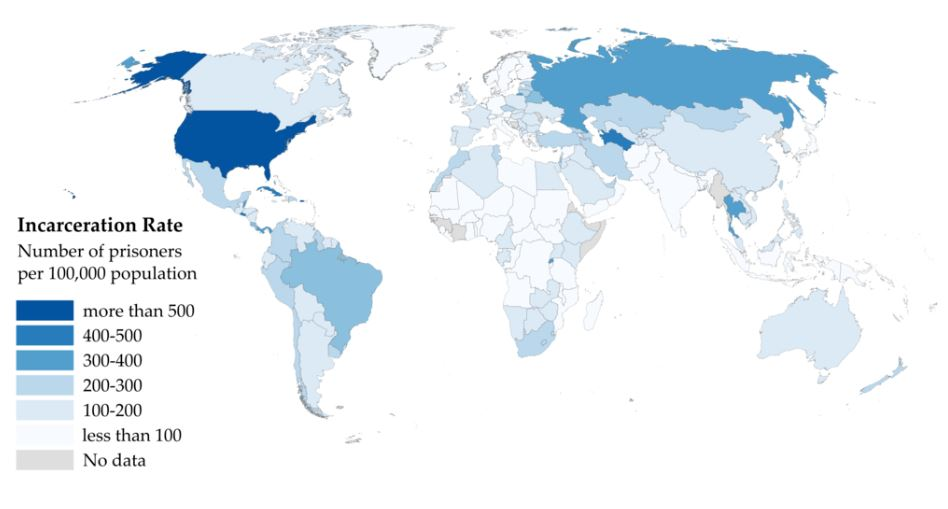
\includegraphics[width=\textwidth]{prison}
\end{figure}
 \end{frame}

%------------------------------------------------

\section{Motivation}
\begin{frame}{Motivation}
    \begin{itemize}
        \item Keeping prisons is very costly
        \item Yet, it can bears even higher cost if criminals are not isolated from society
        \item On the other hand, given brutality and psychologically destructive effects of prison on individuals, prisons might stimulate people to commit crimes in the future over and over again.
        \item So, are the other punishment tools that is more efficient compared to prison?
    \end{itemize}
\end{frame}
%------------------------------------------------
\begin{frame}{Motivation}
    \begin{itemize}
        \item Probably the most widespread substitution for imprisonment is Electronic Monitoring (EM) of convicted individuals.
\begin{figure}        
\centering
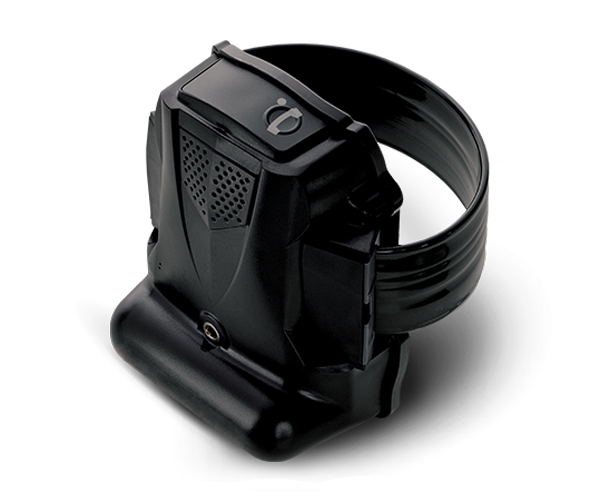
\includegraphics[width=0.3\textwidth]{EM.jpg}
\end{figure}

\item But is it worth to implement EM? What are the risks and who should receive them instead of imprisonment?
\end{itemize}
\end{frame}
%------------------------------------------------

\begin{frame}{Motivation}
   
\begin{figure}
\begin{subfigure}
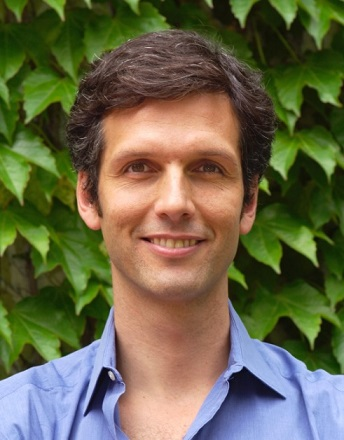
\includegraphics[width=0.3\textwidth, left]{DiTella.jpg}
\end{subfigure}
\begin{subfigure}
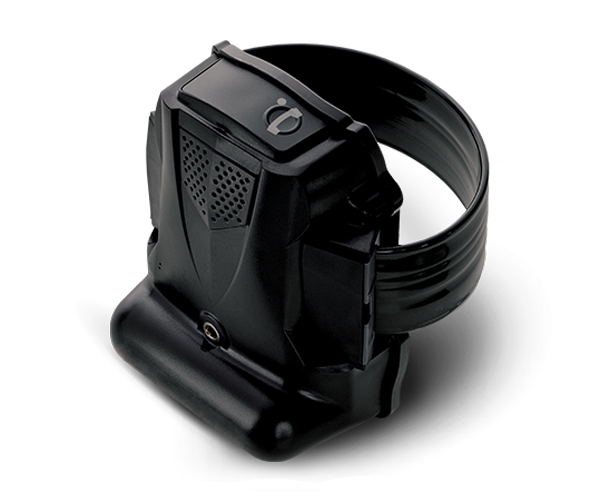
\includegraphics[width=0.3\textwidth, right]{EM.jpg}
\end{subfigure}        
\end{figure}
\begin{center}
 Authors of \textit{"Criminal Recidivism after Electronic Monitoring and Imprisonment"} (JPE, 2013)   
\end{center}
\end{frame}
%------------------------------------------------
\section{Summary of the Original Work}
\begin{frame}{Summary of the paper}
\begin{itemize}
        \item Authors use data from Buenos-Aires Province of Argentina to see whether electronic monitoring indeed helps to reduce recidivism
        \item 
        \item There is a large, negative effect on criminal recidivism of treatment individual with electronic monitoring relative to prison. 
    \end{itemize}
\end{frame}
%------------------------------------------------
\section{Replication}
\begin{frame}{Data and Replication Tools}
\begin{itemize}
    \item Datasets: Obtained from the University of Chicago website \item STATA versions: 14.0 &  15.1 SE
\end{itemize}
\end{frame}
%------------------------------------------------
\begin{frame}{Replication steps}
 \begin{itemize}
    \item 
    \item matching
    \item 
    \item 
\end{itemize}
\end{frame}
%------------------------------------------------
\begin{frame}{ Example}

\end{frame}
%------------------------------------------------
\begin{frame}{Further slides}
You can type smth. here
\begin{itemize}
    \item 1
    \item 2
    \begin{itemize}
        \item separable
        \item minimality
    \end{itemize}
    \item Text 1
    \item Text 2
    \begin{block}{Lemma 2}
    For any superbubble (x,y) in a digraph D, the pair set {x' = (x,right),y'=(y,left)} is an ultrabubble in B(D), a biedged graph
    \end{block}
\end{itemize}
\end{frame}
\section{Measurement Analysis}
\begin{frame}{Measurement Analysis}
    \begin{itemize}
        \item D
        \item E
        \item S
    \end{itemize}
\end{frame}
%------------------------------------------------
\begin{frame}
\frametitle{Blocks of Highlighted Text}
\begin{block}{Block 1}
Lorem ipsum dolor sit amet, consectetur adipiscing elit. Integer lectus nisl, ultricies in feugiat rutrum, porttitor sit amet augue. Aliquam ut tortor mauris. Sed volutpat ante purus, quis accumsan dolor.
\end{block}

\begin{block}{Block 2}
Pellentesque sed tellus purus. Class aptent taciti sociosqu ad litora torquent per conubia nostra, per inceptos himenaeos. Vestibulum quis magna at risus dictum tempor eu vitae velit.
\end{block}
\end{frame}
%------------------------------------------------
\section{Theory of Change}
\begin{frame}{Theory of Change}
    \begin{itemize}
        \item A
        \item B
        \item C
    \end{itemize}
\end{frame}
%------------------------------------------------
\section{Further Extensions}
\begin{frame}{Extensions}
    \begin{itemize}
        \item A
        \item B
        \item C
    \end{itemize}
\end{frame}
%------------------------------------------------
\begin{frame}
\frametitle{References}
\footnotesize{
\begin{thebibliography}{99} % Beamer does not support BibTeX so references must be inserted manually as below
\bibitem[Smith, 2012]{p1} John Smith (2012)
\newblock Title of the publication
\newblock \emph{Journal Name} 12(3), 45 -- 678.
\end{thebibliography}
}
\end{frame}
%------------------------------------------------
\begin{frame}
\Huge{\centerline{Thank you for your attention}}
\end{frame}
%------------------------------------------------
%------------------------------------------------
\end{document}

